\chapter{Những kiến thức nền tảng trong một mô hình phát hiện bất thường ở điện tâm đồ}
\newpage

\section{Kỹ thuật lọc nhiễu Butterworth}
Bộ lọc Butterworth là một loại bộ lọc xử lý tín hiệu được thiết kế để có đáp ứng tần số càng phẳng càng tốt trong băng thông. Nó cũng được gọi là một bộ lọc cường độ phẳng tối đa. Nó được mô tả lần đầu tiên vào năm 1930 bởi kỹ sư và nhà vật lý người Anh Stephen Butterworth trong bài báo của ông có tựa đề "Về lý thuyết của bộ khuếch đại bộ lọc".
\section{Kỹ thuật ngưỡng kích ứng thích hợp}

\section{Mạng Neural Hồi quy (RNN)}
\subsection{Giới thiệu}
Con người không bắt đầu suy nghĩ của họ từ đầu tại tất cả các thời điểm. Cũng như bạn đang đọc bài viết này, bạn hiểu mỗi chữ ở đây dựa vào từ bạn đã hiểu các chữ trước đó chứ không phải là đọc tới đâu ném hết đi tới đó, rồi lại bắt đầu suy nghĩ lại từ đầu tới chữ bạn đang đọc. Tức là tư duy đã có một bộ nhớ để lưu lại những gì diễn ra trước đó.\\
Tuy nhiên các mô hình mạng nơ-ron truyền thống thì không thể làm được việc đó, đó có thể coi là một khuyết điểm chính của mạng nơ-ron truyền thống. Ví dụ, bạn muốn phân loại các bối cảnh xảy ra ở tất cả các thời điểm trong một bộ phim, thì đúng là không rõ làm thế nào để có thể hiểu được một tình huống trong phim mà lại phụ thuộc vào các tình huống trước đó nếu sử dụng các mạng nơ-ron truyền thống.\\
Mạng nơ-ron hồi quy (Recurrent Neural Network) sinh ra để giải quyết vấn đề đó. Mạng này chứa các vòng lặp bên trong cho phép thông tin có thể lưu lại được.
\begin{center}
    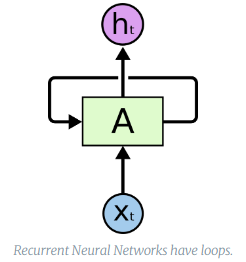
\includegraphics[scale=.5]{image/chapter6/RNN-node.png}
    \begin{figure}[htp]
    \begin{center}
    \end{center}
    \caption{một đoạn của mạng nơ-ron hồi quy A với đầu vào là $x_{n}$ và đầu ra là $h_{t}$. Một vòng lặp cho phép thông tin có thể được truyền từ bước này qua bước này qua bước khác của mạng nơ-ron. \cite{rnn-basic}}
    \end{figure}
\end{center}
Một mạng nơ-ron hồi quy có thể được coi là nhiều bản sao chép của cùng một mạng, trong đó mỗi đầu ra của mạng này là đầu vào của một mạng sao chép khác.\par
\begin{center}
    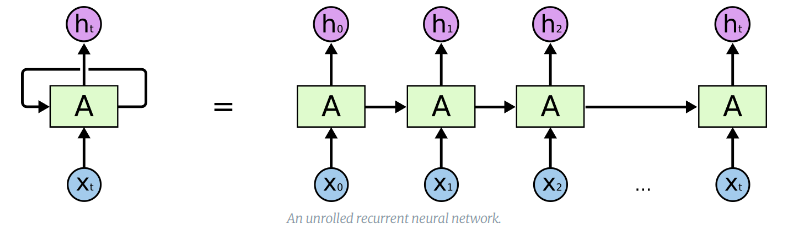
\includegraphics[scale=.5]{image/chapter6/RNN-ab.png}
    \begin{figure}[htp]
    \begin{center}
     
    \end{center}
    \caption{Chuỗi lặp lại các mạng này chính là phân giải của mạng nơ-ron hồi quy, các vòng lặp khiến chúng tạo thành một chuỗi danh sách các mạng sao chép nhau. \cite{rnn-basic}}
    \end{figure}
\end{center}
Một cách chi tiết hơn.
\begin{center}
    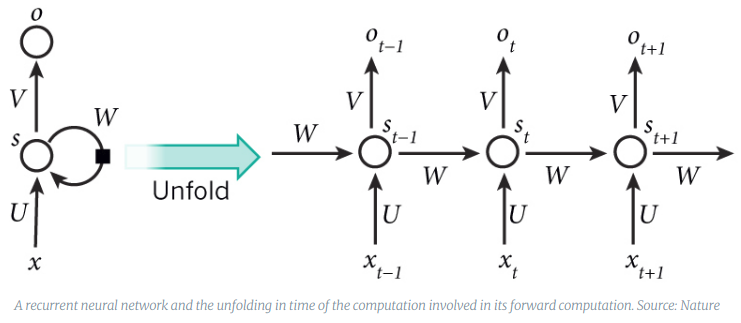
\includegraphics[scale=.4]{image/chapter6/rnn-detail.png}
    \begin{figure}[htp]
    \begin{center}
     
    \end{center}
    \caption{Chi tiết mạng RNN \cite{rnn-basic}}
    \end{figure}
\end{center}
\begin{itemize}
    \item $x_{t}$ là đầu vào tại bước t.
    \item $s_{t}$ là trạng thái ẩn tại bước t. Nó chính là bộ nhớ của mạng. $s_{t}$ được tính toán dựa trên cả các trạng thái ẩn phía trước và đầu vào tại bước đó: $s_{t} = f(Ux_{t}+Ws_{t-1})$. Hàm $f$ thường là một hàm phi tuyến như tang hyperbolic (tanh) hay Relu. Để làm phép toán cho phần tử ẩn đầu tiên ta cần khởi tạo thêm $s_{-1}$, thường giá trị khởi tạo được gắn bằng 0.
    \item $o_{t}$ là đầu ra tại bước t. Ví dụ, ta muốn dự đoán từ tiếp theo có thể xuất hiện trong câu thì $o_{t}$ chính là một vec-tơ xác xuất các từ trong danh sách từ vựng của ta: $o_{t} = softmax(Vs_{t})$. 
\end{itemize}


\subsection{Một số ứng dụng của RNN}
\begin{itemize}
    \item Nhận dạng giọng nói: Đưa vào một chuỗi các tín hiệu âm thanh, ta có thể dự đoán được chuỗi các đoạn ngữ âm đi kèm với xác xuất của chúng.
    \item Mô tả hình ảnh: Cùng với ConvNet, RNN được sử dụng để tự động tạo mô tả cho các ảnh chưa được gán nhãn. Sự kết hợp này đã đưa ra được các kết quả khá kinh ngạc. Ví dụ như các ảnh dưới đây, các mô tả sinh ra có mức độ chính xác và độ tường tận khá cao.
    \begin{center}
    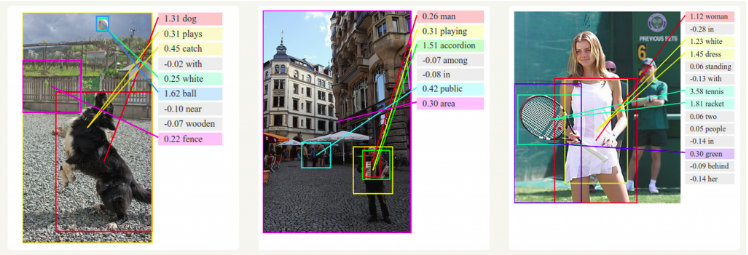
\includegraphics[scale=.4]{image/chapter6/RNN-application.png}
    \begin{figure}[htp]
    \begin{center}
     
    \end{center}
    \caption{Ứng dụng của RNN trong phân loại ảnh \cite{rnn-basic}}
    \end{figure}
    \end{center}
\end{itemize}


\subsection{RNN mở rộng}
\begin{itemize}
    \item RNN 2 chiều: Ở mô hình RNN 2 chiều (Bidirectional RNN), đầu ra tại bước t không những phụ thuộc vào các phần tử phía trước mà còn phụ thuộc cả vào các phần tử phía sau. Ví dụ, để dự đoán từ còn thiếu trong câu, thì việc xem xét cả phần trước và phần sau của câu là cần thiết. Vì vậy, ta có thể coi mô hình là việc chồng 2 mạng RNN ngược hướng nhau lên nhau. Lúc này đầu ra được tính toán dựa vào cả 2 trạng thái ẩn của 2 mạng RNN ngược hướng này.
    \begin{center}
    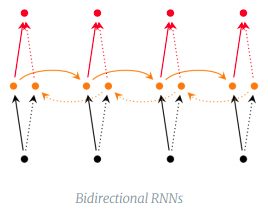
\includegraphics[scale=.5]{image/chapter6/RNN-2.png}
    \begin{figure}[htp]
    \begin{center}
     
    \end{center}
    \caption{RNN 2 chiều \cite{rnn-basic}}
    \end{figure}
    \end{center}
    \item RNN (2 chiều) sâu: RNN sâu (Deep (Bidirectional) RNN) cũng tương tự như RNN 2 chiều, nhưng khác nhau ở chỗ chúng chứa nhiều tầng ẩn ở mỗi bước. Trong thực tế, chúng giúp cho việc học ở mức độ cao hơn, tuy nhiên ta cũng cần phải có nhiều dữ liệu huấn luyện hơn.
    \begin{center}
    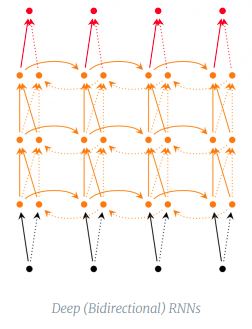
\includegraphics[scale=.3]{image/chapter6/RNN-4.png}
    \begin{figure}[htp]
    \begin{center}
     
    \end{center}
    \caption{RNN sâu \cite{rnn-basic}}
    \end{figure}
    \end{center}
\end{itemize}


\section{Mạng bộ nhớ ngắn dài (LSTM)}
\subsection{Vấn đề phụ thuộc xa}
Một điểm nổi bật của RNN chính là ý tưởng kết nối các thông tin phía trước để dự đoán cho hiện tại. Việc này tương tự như ta sử dụng các cảnh trước của bộ phim để hiểu được cảnh hiện thời. Nếu mà RNN có thể làm được việc đó thì chúng sẽ cực kì hữu dụng, tuy nhiên liệu chúng có thể làm được không? Câu trả lời là còn tùy.\\
Đôi lúc ta chỉ cần xem lại thông tin vừa có thôi là đủ để biết được tình huống hiện tại. Ví dụ, ta có câu: “các đám may trên bầu trời” thì ta chỉ cần đọc tới “các đám may trên bầu” là đủ biết được chữ tiếp theo là “trời” rồi. Trong tình huống này, khoảng cách tới thông tin có được cần để dự đoán là nhỏ, nên RNN hoàn toàn có thể học được.
\begin{center}
    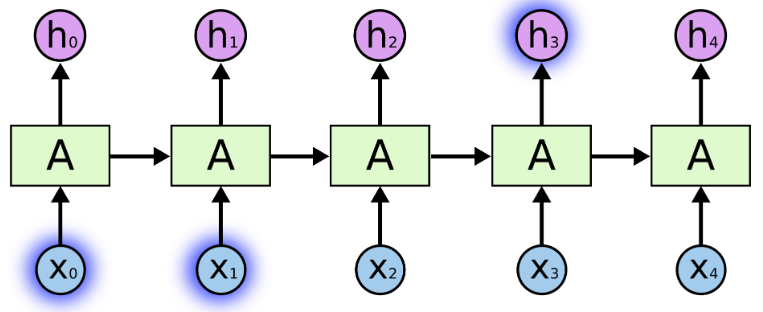
\includegraphics[scale=.3]{image/chapter6/ptx1.png}
    \begin{figure}[htp]
    \begin{center}
     
    \end{center}
    \end{figure}
\end{center}
Nhưng trong nhiều tình huống ta buộc phải sử dụng nhiều ngữ cảnh hơn để suy luận. Ví dụ, dự đoán chữ cuối cùng trong đoạn: “I grew up in France… I speak fluent French.”. Rõ ràng là các thông tin gần (”I speak fluent”) chỉ có phép ta biết được đằng sau nó sẽ là tên của một ngôn ngữ nào đó, còn không thể nào biết được đó là tiếng gì. Muốn biết là tiếng gì, thì ta cần phải có thêm ngữ cảnh “I grew up in France” nữa mới có thể suy luận được. Rõ ràng là khoảng cách thông tin lúc này có thể đã khá xa rồi.\\
Thật không may là với khoảng cách càng lớn dần thì RNN bắt đầu không thể nhớ và học được nữa.
\begin{center}
    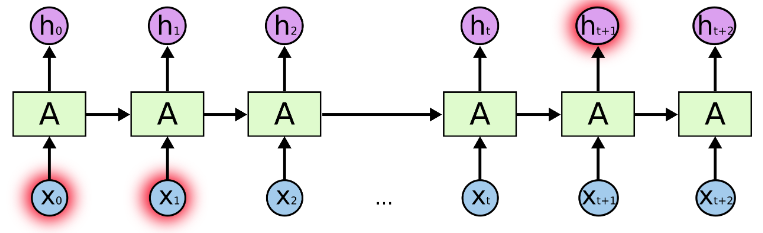
\includegraphics[scale=.3]{image/chapter6/ptx2.png}
    \begin{figure}[htp]
    \begin{center}
     
    \end{center}
    \end{figure}
\end{center}
Về mặt lý thuyết, rõ ràng là RNN có khả năng xử lý các phụ thuộc xa (long-term dependencies). Chúng ta có thể xem xét và cài đặt các tham số sao cho khéo là có thể giải quyết được vấn đề này. Tuy nhiên, đáng tiếc trong thực tế RNN có vẻ không thể học được các tham số đó. Vấn đề này đã được khám phá khá sâu bởi Hochreiter (1991) [tiếng Đức] và Bengio, et al. (1994), trong các bài báo của mình, họ đã tìm được nhưng lý do căn bản để giải thích tại sao RNN không thể học được.


\subsection{Mạng LSTM}
Mạng bộ nhớ dài-ngắn (Long Short Term Memory networks), thường được gọi là LSTM - là một dạng đặc biệt của RNN, nó có khả năng học được các phụ thuộc xa. LSTM được giới thiệu bởi Hochreiter và Schmidhuber (1997), và sau đó đã được cải tiến và phổ biến bởi rất nhiều người trong ngành. Chúng hoạt động cực kì hiệu quả trên nhiều bài toán khác nhau nên dần đã trở nên phổ biến như hiện nay.\\
LSTM được thiết kế để tránh được vấn đề phụ thuộc xa (long-term dependency). Việc nhớ thông tin trong suốt thời gian dài là đặc tính mặc định của chúng, chứ ta không cần phải huấn luyện nó để có thể nhớ được. Tức là ngay nội tại của nó đã có thể ghi nhớ được mà không cần bất kì can thiệp nào.\\
Mọi mạng hồi quy đều có dạng là một chuỗi các mô-đun lặp đi lặp lại của mạng nơ-ron. Với mạng RNN chuẩn, các mô-dun này có cấu trúc rất đơn giản, thường là một tầng $tanh$
\begin{center}
    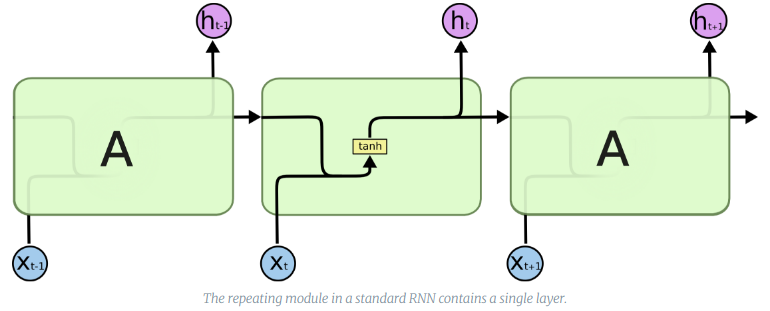
\includegraphics[scale=.3]{image/chapter6/lstm1.png}
    \begin{figure}[htp]
    \begin{center}
    \end{center}
    \end{figure}
\end{center}
LSTM cũng có kiến trúc dạng chuỗi như vậy, nhưng các mô-đun trong nó có cấu trúc khác với mạng RNN chuẩn. Thay vì chỉ có một tầng mạng nơ-ron, chúng có tới 4 tầng tương tác với nhau một cách rất đặc biệt.
\begin{center}
    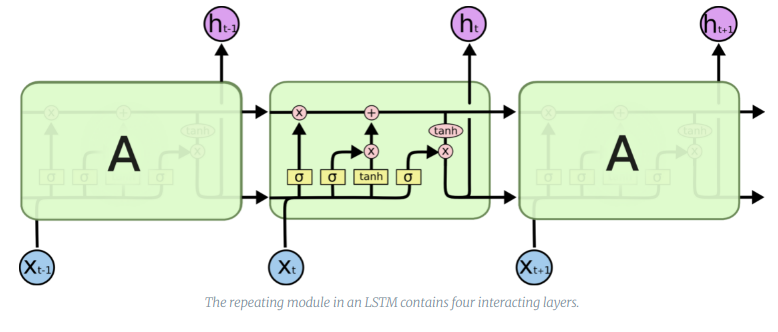
\includegraphics[scale=.3]{image/chapter6/lstm2.png}
    \begin{figure}[htp]
    \begin{center}
     
    \end{center}
    \end{figure}
\end{center}
Giờ thì đừng hoang mang về chi tiết bên trong chúng ngay, chúng ta sẽ khám phá chúng chi tiết chúng ở bước sau. Điều bạn cần làm bây giờ là làm hãy làm quen với các kí hiệu mà ta sẽ sử dụng ở dưới đây:
\begin{center}
    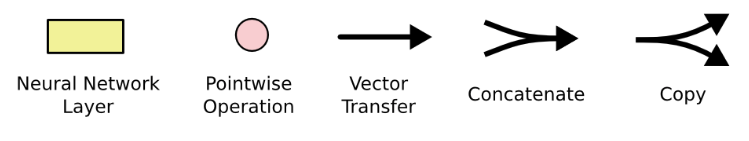
\includegraphics[scale=.3]{image/chapter6/lstm3.png}
    \begin{figure}[htp]
    \begin{center}
     
    \end{center}
    \end{figure}
\end{center}
Ở sơ đồ trên, mỗi một đường mang một véc-tơ từ đầu ra của một nút tới đầu vào của một nút khác. Các hình trong màu hồng biểu diễn các phép toán như phép cộng véc-tơ chẳng hạn, còn các ô màu vàng được sử dụng để học trong các từng mạng nơ-ron. Các đường hợp nhau kí hiệu việc kết hợp, còn các đường rẽ nhánh ám chỉ nội dung của nó được sao chép và chuyển tới các nơi khác nhau.


\subsection{Ý tưởng cốt lõi của LSTM}
Chìa khóa của LSTM là trạng thái tế bào (cell state) - chính đường chạy thông ngang phía trên của sơ đồ hình vẽ.\par
Trạng thái tế bào là một dạng giống như băng truyền. Nó chạy xuyên suốt tất cả các mắt xích (các nút mạng) và chỉ tương tác tuyến tính đôi chút. Vì vậy mà các thông tin có thể dễ dàng truyền đi thông suốt mà không sợ bị thay đổi.
\begin{center}
    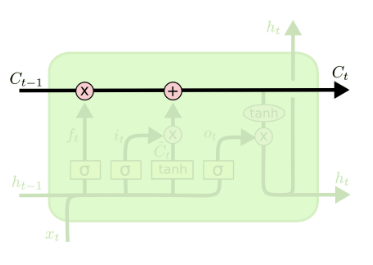
\includegraphics[scale=.5]{image/chapter6/yn1.png}
    \begin{figure}[htp]
    \begin{center}
     
    \end{center}
    \end{figure}
\end{center}
LSTM có khả năng bỏ đi hoặc thêm vào các thông tin cần thiết cho trạng thái tế báo, chúng được điều chỉnh cẩn thận bởi các nhóm được gọi là cổng (gate).\par
Các cổng là nơi sàng lọc thông tin đi qua nó, chúng được kết hợp bởi một tầng mạng sigmoid và một phép nhân.
\begin{center}
    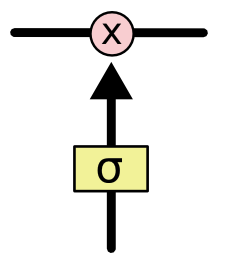
\includegraphics[scale=.3]{image/chapter6/yn2.png}
    \begin{figure}[htp]
    \begin{center}
     
    \end{center}
    \end{figure}
\end{center}
Tầng sigmoid sẽ cho đầu ra là một số trong khoản [0,1], mô tả có bao nhiêu thông tin có thể được thông qua. Khi đầu ra là 0 thì có nghĩa là không cho thông tin nào qua cả, còn khi là 1 thì có nghĩa là cho tất cả các thông tin đi qua nó.\\
Một LSTM gồm có 3 cổng như vậy để duy trì và điều hành trạng thái của tế bào.
\subsection{Bên trong LSTM}
Bước đầu tiên của LSTM là quyết định xem thông tin nào cần bỏ đi từ trạng thái tế bào. Quyết định này được đưa ra bởi tầng sigmoid - gọi là “tầng cổng quên” (forget gate layer). Nó sẽ lấy đầu vào là $h_{t-1}$ và $x_{t}$ rồi đưa ra kết quả là một số trong khoảng [0,1] cho mỗi số trong trạng thái tế bào $C_{t-1}$ Đẩu ra là 1 1 thể hiện rằng nó giữ toàn bộ thông tin lại, còn 0 chỉ rằng toàn bộ thông tin sẽ bị bỏ đi.\\
Quay trở lại với ví dụ mô hình ngôn ngữ dự đoán từ tiếp theo dựa trên tất cả các từ trước đó, với những bài toán như vậy, thì trạng thái tế bào có thể sẽ mang thông tin về giới tính của một nhân vật nào đó giúp ta sử dụng được đại từ nhân xưng chuẩn xác. Tuy nhiên, khi đề cập tới một người khác thì ta sẽ không muốn nhớ tới giới tính của nhân vật nữa, vì nó không còn tác dụng gì với chủ thế mới này.
\begin{center}
    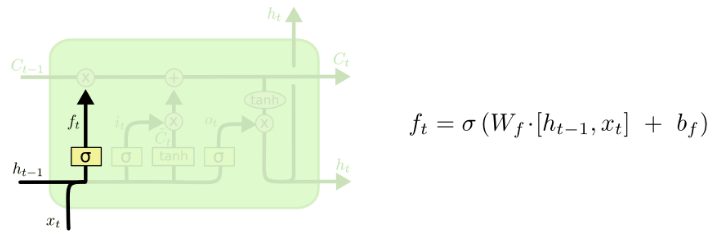
\includegraphics[scale=.5]{image/chapter6/bt1.png}
    \begin{figure}[htp]
    \begin{center}
     
    \end{center}
    \end{figure}
\end{center}
Bước tiếp theo là quyết định xem thông tin mới nào ta sẽ lưu vào trạng thái tế bào. Việc này gồm 2 phần. Đầu tiên là sử dụng một tầng sigmoid được gọi là “tầng cổng vào” (input gate layer) để quyết định giá trị nào ta sẽ cập nhập. Tiếp theo là một tầng $tanh$ tạo ra một véc-tơ cho giá trị mới $\widetilde{C}_{t}$ nhằm thêm vào cho trạng thái. Trong bước tiếp theo, ta sẽ kết hợp 2 giá trị đó lại để tạo ra một cập nhập cho trạng thái.\\
Chẳng hạn với ví dụ mô hình ngôn ngữ của ta, ta sẽ muốn thêm giới tính của nhân vật mới này vào trạng thái tế bào và thay thế giới tính của nhân vật trước đó.
\begin{center}
    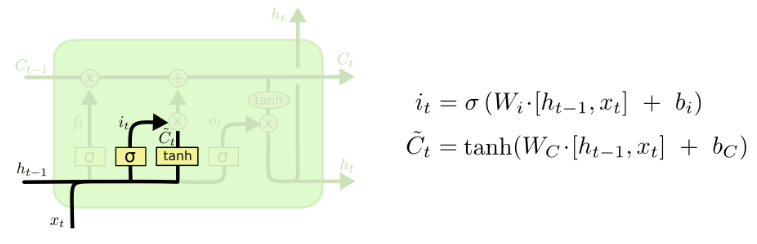
\includegraphics[scale=.5]{image/chapter6/bt2.png}
    \begin{figure}[htp]
    \begin{center}
     
    \end{center}
    \end{figure}
\end{center}
Giờ là lúc cập nhập trạng thái tế bào cũ $C_{t-1}$ thành trạng thái mới $C_{t}$ Ở các bước trước đó đã quyết định những việc cần làm, nên giờ ta chỉ cần thực hiện là xong.\\
Ta sẽ nhân trạng thái cũ với $f_{t}$ để bỏ đi những thông tin ta quyết định quên lúc trước. Sau đó cộng thêm $i_{t} * \widetilde{C}_{t}$. Trạng thái mơi thu được này phụ thuộc vào việc ta quyết định cập nhập mỗi giá trị trạng thái ra sao.\\
Với bài toàn mô hình ngôn ngữ, chính là việc ta bỏ đi thông tin về giới tính của nhân vật cũ, và thêm thông tin về giới tính của nhân vật mới như ta đã quyết định ở các bước trước đó.
\begin{center}
    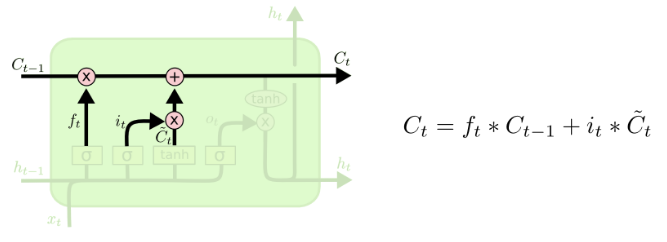
\includegraphics[scale=.5]{image/chapter6/bt3.png}
    \begin{figure}[htp]
    \begin{center}
     
    \end{center}
    \end{figure}
\end{center}
Cuối cùng, ta cần quyết định xem ta muốn đầu ra là gì. Giá trị đầu ra sẽ dựa vào trạng thái tế bào, nhưng sẽ được tiếp tục sàng lọc. Đầu tiên, ta chạy một tầng sigmoid để quyết định phần nào của trạng thái tế bào ta muốn xuất ra. Sau đó, ta đưa nó trạng thái tế bảo qua một hàm tanh để co giá trị nó về khoảng [-1, 1], và nhân nó với đầu ra của cổng sigmoid để được giá trị đầu ra ta mong muốn.\par
Với ví dụ về mô hình ngôn ngữ, chỉ cần xem chủ thể mà ta có thể đưa ra thông tin về một trạng từ đi sau đó. Ví dụ, nếu đầu ra của chủ thể là số ít hoặc số nhiều thì ta có thể biết được dạng của trạng từ đi theo sau nó phải như thế nào.
\begin{center}
    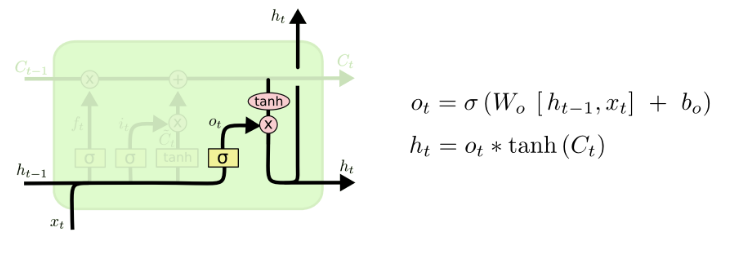
\includegraphics[scale=.5]{image/chapter6/bt4.png}
    \begin{figure}[htp]
    \begin{center}
     
    \end{center}
    \end{figure}
\end{center}


\subsection{Các biến thể của bộ nhớ dài hạn}
Những thứ ta vừa mô tả ở trên là một LSTM khá bình thường. Nhưng không phải tất cả các LTSM đều giống như vậy. Thực tế, các bài báo về LTSM đều sử dụng một phiên bản hơi khác so với mô hình LTSM chuẩn. Sự khác nhau không lớn, nhưng chúng giúp giải quyết phần nào đó trong cấu trúc của LTSM.\\
Một dạng LTSM phổ biến được giới thiệu bởi Gers và Schmidhuber (2000) được thêm các đường kết nối “peephole connections”, làm cho các tầng cổng nhận được giá trị đầu vào là trạng thái tế bào.
\begin{center}
    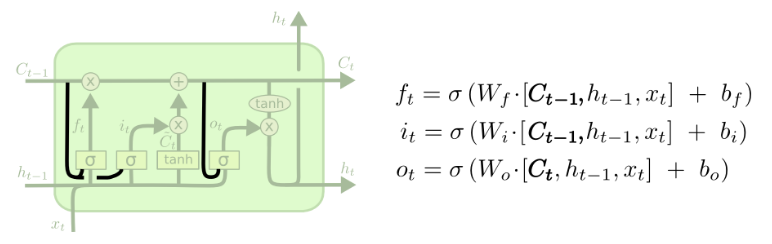
\includegraphics[scale=.5]{image/chapter6/bth1.png}
    \begin{figure}[htp]
    \begin{center}
     
    \end{center}
    \caption{Hình trên mô tả các đường được thêm vào mọi cổng, nhưng cũng có những bài báo chỉ thêm cho một vài cổng mà thôi.}
    \end{figure}
\end{center}
Một biến thể khác là nối 2 cổng loại trừ và đầu vào với nhau. Thay vì phân tách các quyết định thông tin loại trừ và thông tin mới thêm vào, ta sẽ quyết định chúng cùng với nhau luôn. Ta chỉ bỏ đi thông tin khi mà ta thay thế nó bằng thông tin mới đưa vào. Ta chỉ đưa thông tin mới vào khi ta bỏ thông tin cũ nào đó đi.
\begin{center}
    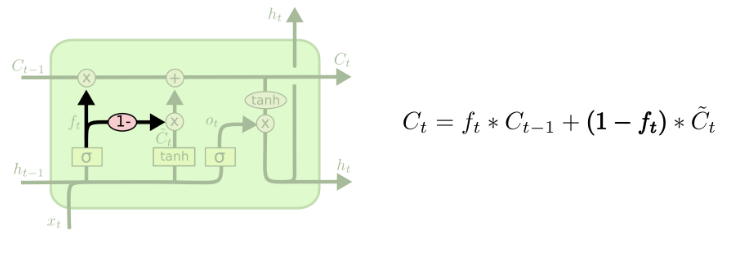
\includegraphics[scale=.5]{image/chapter6/bth2.png}
    \begin{figure}[htp]
    \begin{center}
     
    \end{center}
    \end{figure}
\end{center}
Một biến thể khá thú vị khác của LSTM là Gated Recurrent Unit, hay GRU được giới thiệu bởi Cho, et al. (2014). Nó kết hợp các cổng loại trừ và đầu vào thành một cổng “cổng cập nhập” (update gate). Nó cũng hợp trạng thái tế bào và trạng thái ẩn với nhau tạo ra một thay đổi khác. Kết quả là mô hình của ta sẽ đơn giản hơn mô hình LSTM chuẩn và ngày càng trở nên phổ biến.
\begin{center}
    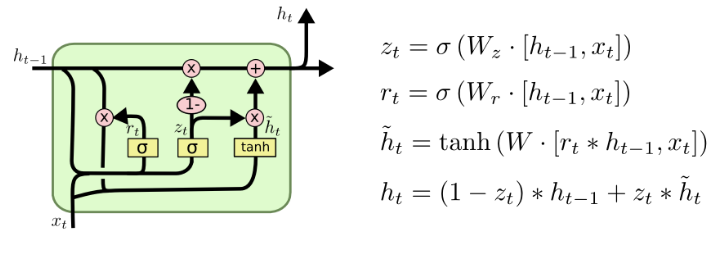
\includegraphics[scale=.5]{image/chapter6/bth3.png}
    \begin{figure}[htp]
    \begin{center}
     
    \end{center}
    \end{figure}
\end{center}
Trên đây chỉ là một vài biến thế được chú ý nhiều nhất thôi, thực tế có rất nhiều các biến thể khác nhau của LSTM như Depth Gated RNNs của Yao, et al. (2015). Cũng có những biến thể mà chiến lực xử lý phụ thuộc xa hoàn toàn khác như Clockwork RNNs của Koutnik, et al. (2014).\\
Nếu bạn muốn tìm hiểu xem biến thể nào là tốt nhất và chúng khác nhau thế nào, thì có thể đọc bài so sánh khá hay này của Greff, et al. (2015). Ngoài ra thì Jozefowicz, et al. (2015) thậm chí còn thử hàng chục nghìn kiến trúc RNN khác nhau và tìm ra một vài mô hình hoạt động tốt hơn cả LSTM ở một số bài toán.


\section{Kết luận}
RNN đặc biệt là LSTM được sử dụng nhiều trong những bài toán về chuỗi dữ liệu: mô hình ngôn ngữ, nhận dạng giọng nói,... Theo bài báo của Shraddha Singh và nhóm nghiên cứu mạng LSTM đem lại kết quả tốt nhất trong số 3 biến thể của RNN trong phân loại ECG-phát hiện đoạn run nhĩ RNN-acc:85.4\%, GRU-acc:82.5\%, LSTM-acc: 88.1\% \cite{ketluanlstm}.
